\chapter{The RAW Dataset}\label{ch:benchmarks_and_metrics}
In this chapter the RAW dataset is going to be presented. This dataset has been produced as a requirement of the FlexSight\footnote{http://www.flexsight.eu/} project. FlexSight is a research project founded by the European Community's project ECHORD++\footnote{http://echord.eu/}.  This project involves three main partners: the Ro.Co.Co. Laboratory\footnote{http://www.dis.uniroma1.it/~labrococo/} of DIAG (Department of Computer, Control, and Management Engineering  Antonio Ruberti at Sapienza University of Rome), which provides expertise in software design and development for robotic perception applications; IT+Robotics\footnote{http://www.it-robotics.it/}, which provides expertise in the industrial robotics domain; and Robox\footnote{http://www.robox.it/en-US/}, a company specialized in the development of innovative hardware and software solutions for robotics and control systems. 

More details about the FlexSight project can be found in the Appendix \ref{apx:flexsight} of this thesis.

\section{RAW Dataset Features}\label{sec:raw_features}
As like as the previous datasets presented in sections \ref{subsec:mvtex_itodd} and \ref{subsec:tless_dataset} also the RAW Dataset has been built for industrial scenarios. The main scope of the RAW Dataset is to build a large and consistent test bed for texture-less object detection and localization algorithms. The name of the dataset is related to the RoboCup@Work competition, which more details are given in the Appendix \ref{apx:robocupatwork}, and it contains all the objects used in the robotic competition plus other objects from other past robotics events, such as the RoCKIn@Work\footnote{http://rockinrobotchallenge.eu/} (Robot Competitions Kick Innovation in Cognitive Systems and Robotics) and ERL\footnote{https://www.eu-robotics.net/robotics\_league/index.html} (European Robotics League). 

As already mentioned, all the objects present in the dataset are texture-less objects and are inspired to the industrial settings, e.g. parts of a motor, bearings, nuts, motor axis and others. A compact view of all the objects present in the dataset is given in Figure \ref{fig:raw_obj_examples}, and the complete list of objects with their specific name and class is reported in Table \ref{tab:raw_objs_list}.

\begin{table}
    \centering
    \begin{tabular}{| l | l | l |}
    \hline
    \textbf{Name} & \textbf{Class} & \textbf{Description} \\ \hline
    F20\_20\_B & 0 & Black small aluminium profile \\
    F20\_20\_G & 1 & Gray small aluminium profile \\
    M20 & 2 & Small nut \\
    M20\_100 & 3 & Heavy large screw \\
    M30 & 4 & Big nut \\
    R20 & 5 & Plastic tube with shaped borders \\
    S40\_40\_B & 6 & Black large aluminium profile \\
    S40\_40\_G & 7 & Gray large aluminium profile \\
    V20 & 8 & Plastic tube without shaped borders \\
    Bearing\_box & 9 & Small motor box for bearings \\
    Bearing\_box\_B & 10 & Small motor box for bearings (Type B) \\
    Motor & 11 & Black plastic reconstruction of a motor \\
    Axis & 12 & Aluminium motor axis \\
    Distance\_tube & 13 & Small aluminium ring \\
    Bearing & 14 & Real bearing for motors \\
    Cover\_plate\_NOHOLE & 15 & Thin aluminium plate with hole \\
    Cover\_plate\_HOLE & 16 & Thin aluminium plate without hole \\
    Cover\_plate\_BOX & 17 & Black plastic box for cover plates \\
    Bearing\_box\_BOX & 18 & Black plastic box for bearing boxes \\
    \hline
    \end{tabular}
    \caption{\textbf{The RAW Dataset Objects.} In this table is reported the list of all the objects present in the RAW dataset, with their name, class and a brief description.}
    \label{tab:raw_objs_list}
\end{table}

\begin{figure}
    \centering
    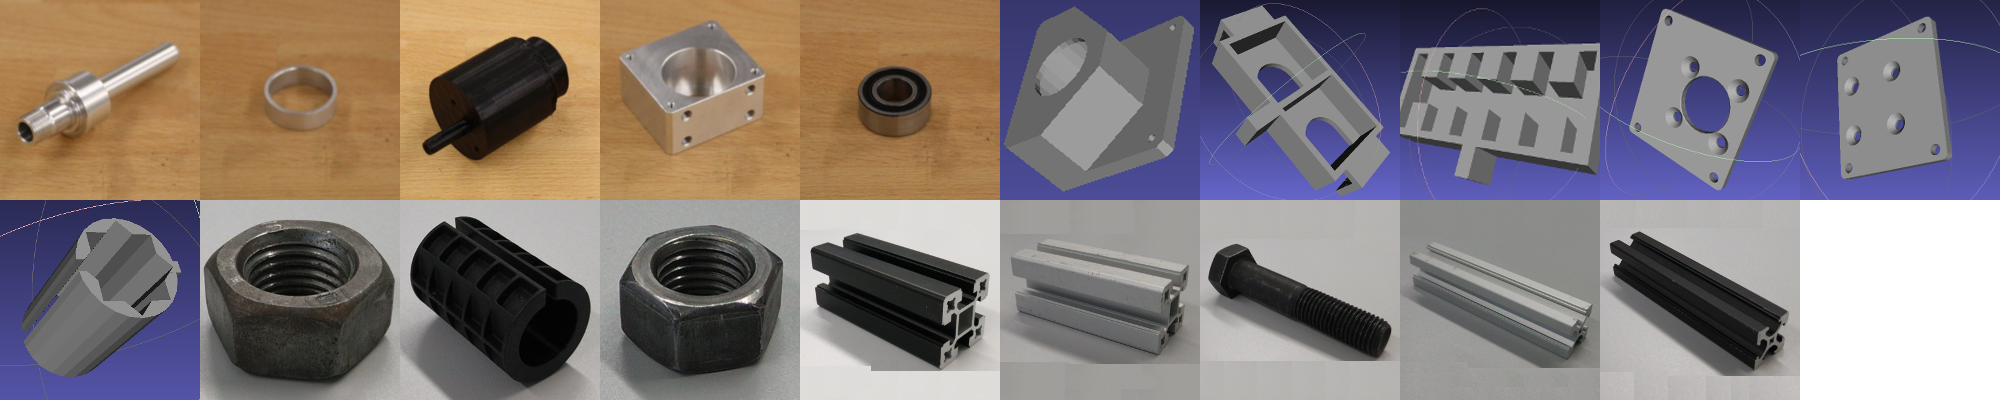
\includegraphics[width=0.9\textwidth]{figures/3_raw_dataset/raw_obj_examples}
    \caption{\textbf{RAW Dataset Objects.} A compact view of all the 19 classes of objects present in the RAW Dataset.}
    \label{fig:raw_obj_examples}
\end{figure}

The main features of this dataset are the following:
\begin{itemize}
	\item \textbf{19 indutry relevant objects}: no discriminative color, no texture, often similar in shape;
	\item \textbf{3 different sensors}: FlexSight sensor, Microsoft Kinect2, Intel RealSense SR-300;
	\item \textbf{Test images (7K from each sensor)}: originated from 15 test scenes. The scene complexity varies from simple scenes with several isolated objects to very challenging ones with multiple object instances and a high amount of clutter and occlusion. Images include: RGB and Depth for Kinect2 and RealSense SR-300; 2 grey-scale images (with and without projected laser pattern) for the FlexSight sensor;
	\item \textbf{19 object 3D CAD models}: all the objects have a specific 3D CAD model.
\end{itemize}

Each image of the dataset comes with ground truth estimate of all the objects present in the scene. The full 3D position in space, rotation plus translation with respect to the camera frame, has been annotated with a specific protocol that involved both manually intervention of the user by means of our own developed labeling tool and some other automatic procedures for propagating the pose in a given reference frame to all the other images of the dataset.

\begin{figure}
    \centering
    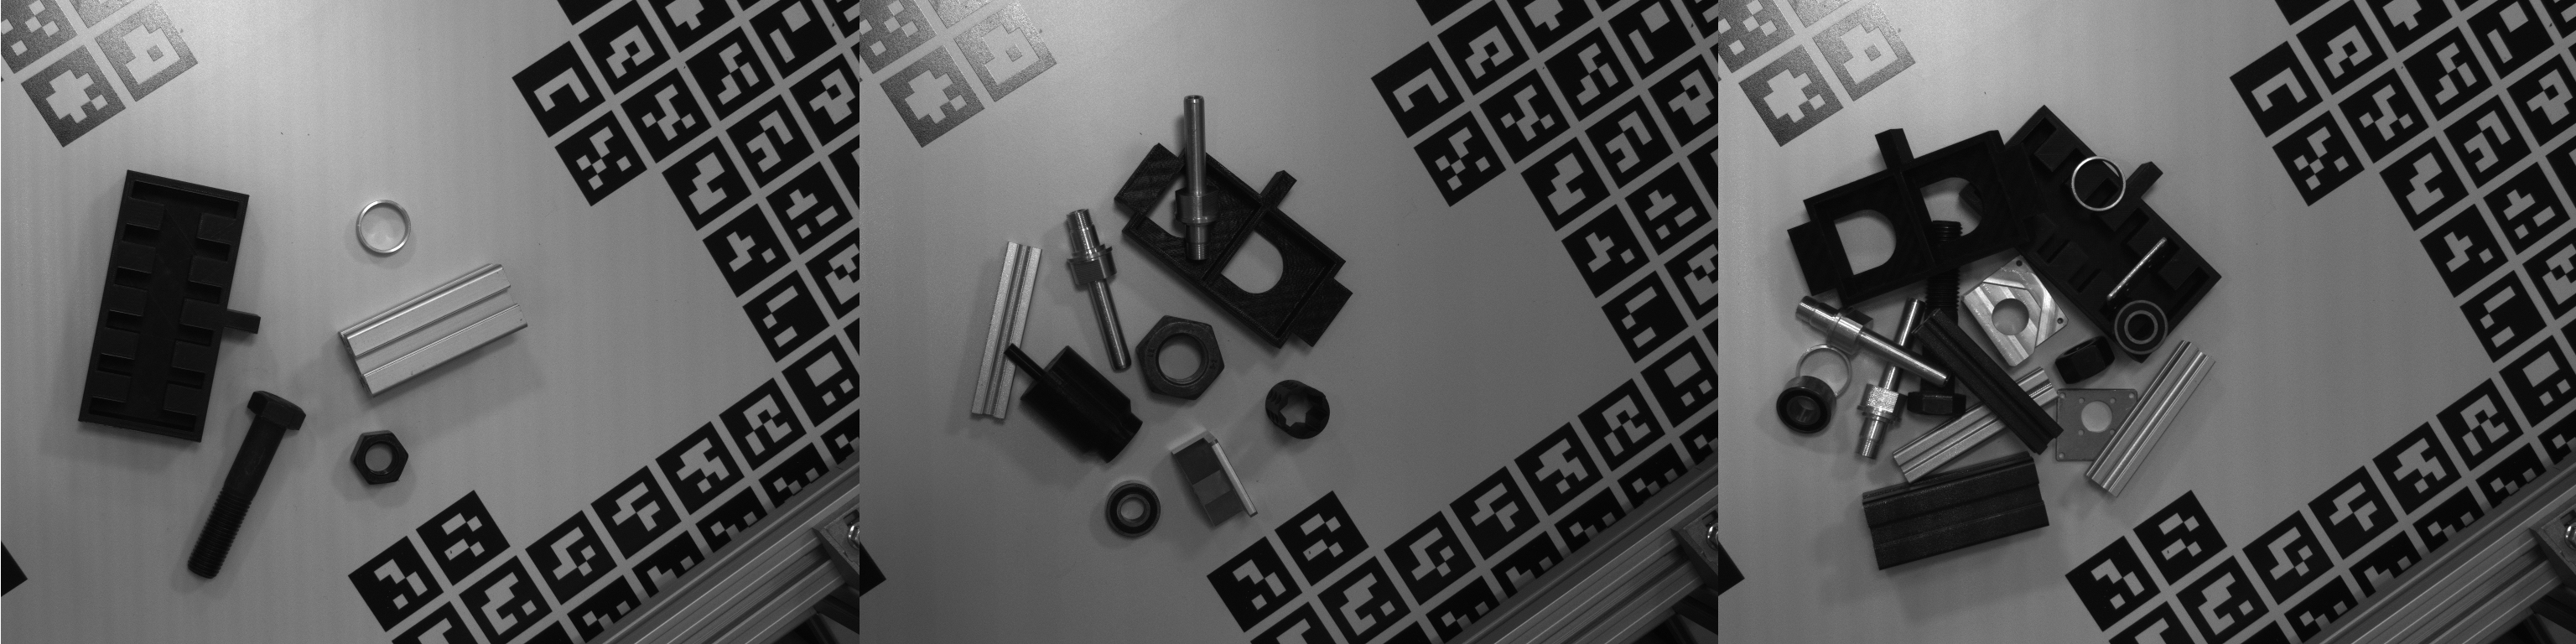
\includegraphics[width=0.9\textwidth]{figures/3_raw_dataset/easy_medium_hard_scene}
    \caption{\textbf{RAW Dataset Scenes Comparison.} From left to right: easy scene, medium scene and hard scene. All the images refers to the camera left of the FlexSight sensor and are without the projected laser pattern.}
    \label{fig:easy_medium_hard_scene}
\end{figure}

\section{Details of the Scenes}\label{sec:raw_scenes_details}
As already anticipated, the RAW Dataset comes with 15 different scenes. In particular, those scenes are aggregated in three different categories: \emph{easy}, \emph{medium} and \emph{hard}. This categorization depends on the level of complexity of the disposition of the objects in the scenes. An example of easy medium and hard scene comparison is given in Figure \ref{fig:easy_medium_hard_scene}. Moreover, easy scenes does not contain any occlusion or overlapping of the objects, while medium and hard scenes do.

Each scene is composed as follow:

\begin{itemize}
	\item \textbf{FlexSight Sensor Data}: 465 images, both for camera left and camera right of the sensor. Each image has been acquired with and without the projected laser pattern (See Figure \ref{fig:flexsight_laser_no_laser_ex}).
	\item \textbf{Microsoft Kinect 2}: 465 rgb-d images. We provide both rgb and depth image, together with the automatic generated registered pointcloud.
	\item \textbf{Intel Realsense SR300}: 465 rgb-d images. For the Intel Realsense SR300 only rgb and depth images are provided.
\end{itemize}

\begin{figure}
    \centering
    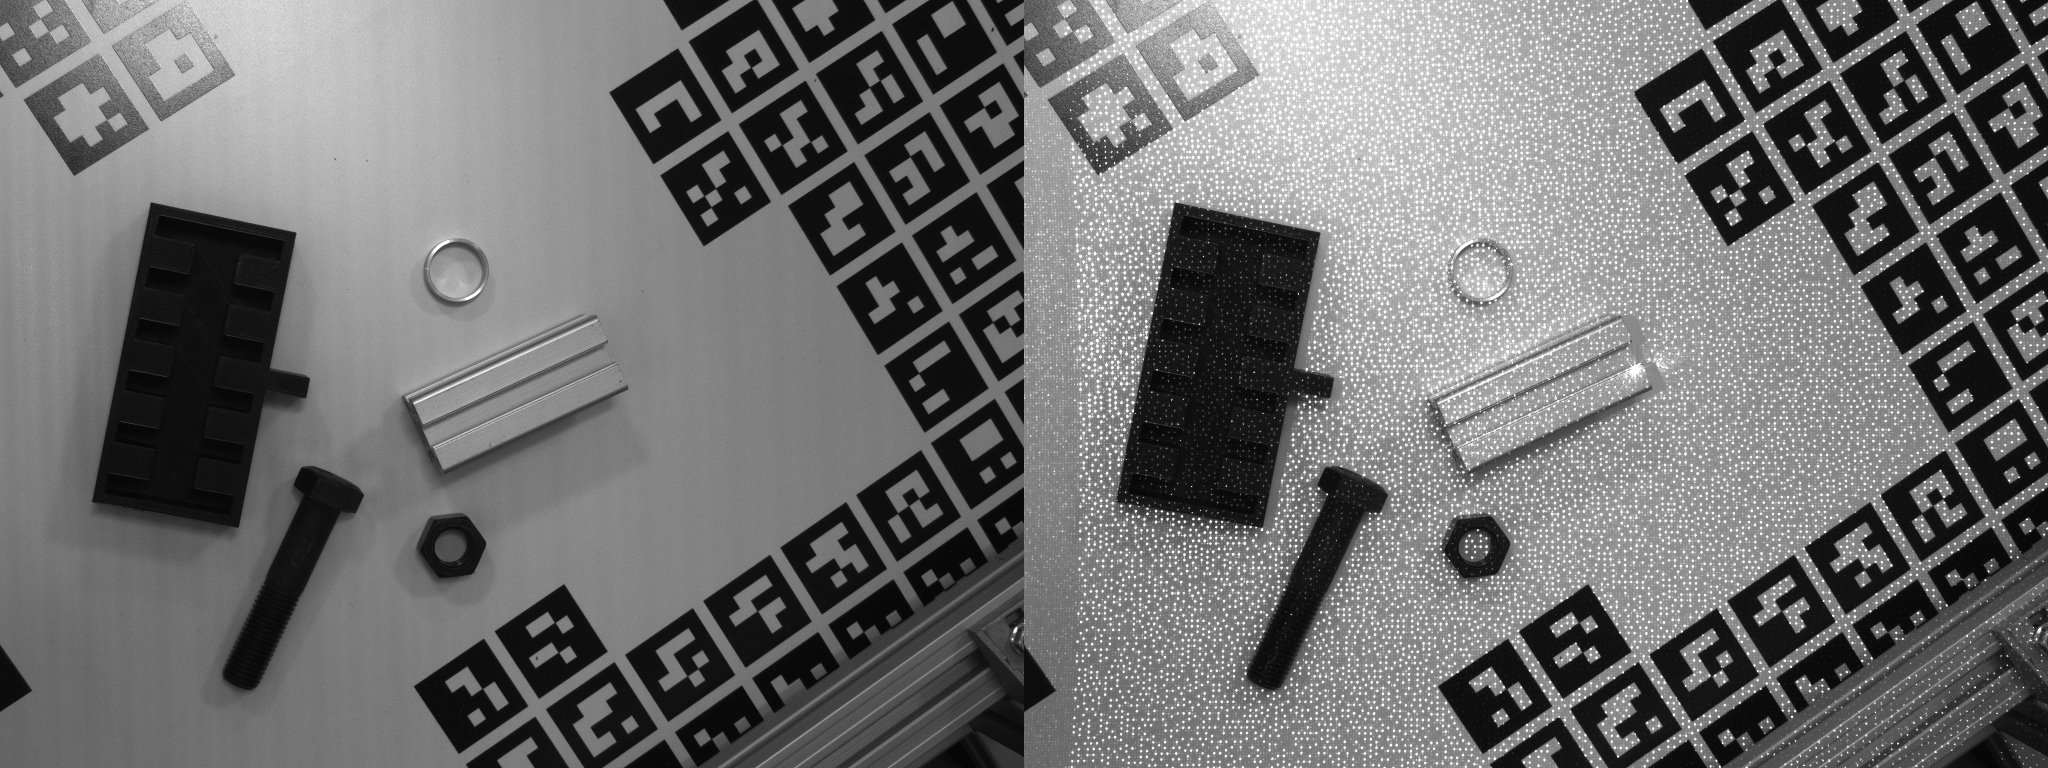
\includegraphics[width=0.9\textwidth]{figures/3_raw_dataset/flexsight_laser_no_laser_ex}
    \caption{\textbf{FlexSight Sensor Acquisition (with and without laser pattern).} On the left the FlexSight Sensor image acquired without projected laser pattern, on the right with projected laser pattern.}
    \label{fig:flexsight_laser_no_laser_ex}
\end{figure}

\section{Setup and Sensors}\label{sec:raw_setup_and_sensors}
As already mentioned in the introduction if this chapter, the RAW Dataset has been acquired in fulfillment of the data acquisition requirement of the FlexSight project. For this scope, a completely new and custom robot-sensors setup has been built in collaboration with the two other partners of the project, IT+Robotics and Robox. This setup consists in a custom built cell with a robotic manipulator inside, which has the experimental sensor mounted at its end-effector. A 3D model view of the robotic cell is given in Figure \ref{fig:raw_cell_example}.

In the following sections the robotic arm and all the sensors will be explained in detail.

\begin{figure}
    \centering
    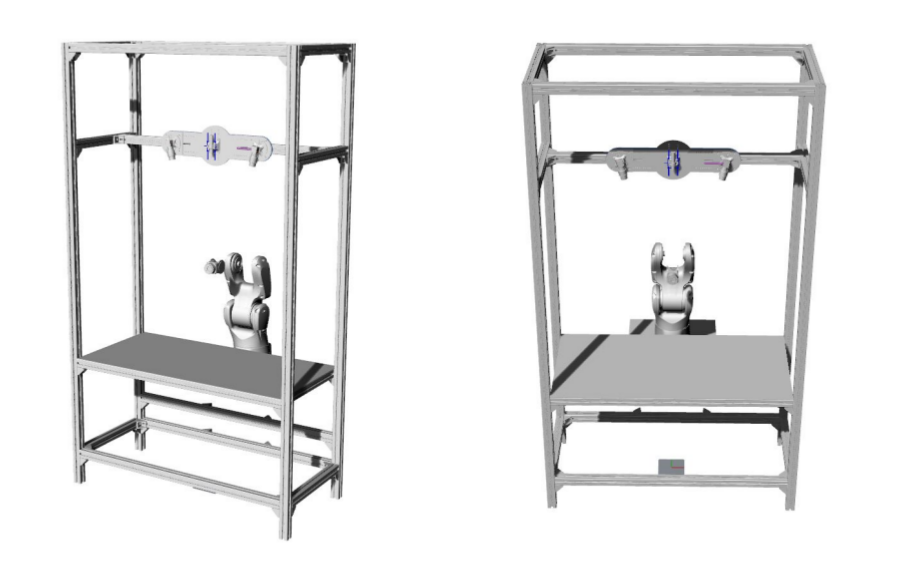
\includegraphics[width=0.9\textwidth]{figures/3_raw_dataset/raw_cell_example}
    \caption{\textbf{FlexSight Robotic Cell 3D Model View.} A 3D reconstruction of the custom robotic cell developed and built for the RAW Dataset acquisition. The figure just reports the robotic cell with the first prototype of the FlexSight sensor mounted on the top and a fake robotic arm as placeholder for the real one.}
    \label{fig:raw_cell_example}
\end{figure}

\subsection{The Robotic Arm}\label{subsec:raw_setup_robot}
The robotic arm used for the acquisition of the RAW Dataset is a 6 d.o.f. robotic manipulator. It has been provided by Robox as contribution to the FlexSight project.The company also provided their own control system with which we interfaced via serial communication for positioning and sending commands to the robot during the acquisition procedure. A picture of the robotic manipulator is given in Figure \ref{fig:raw_robot_example}.

\begin{figure}
    \centering
    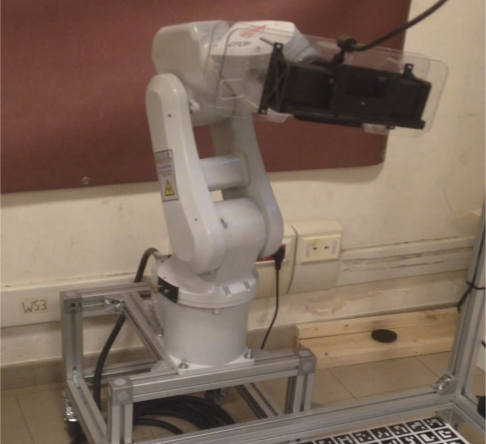
\includegraphics[width=0.8\textwidth]{figures/3_raw_dataset/raw_robot_example}
    \caption{\textbf{FlexSight Robotic Manipulator}. In the picture, the 6 d.o.f. robotic manipulator used for the acquisition of the RAW Dataset scenes.}
    \label{fig:raw_robot_example}
\end{figure}

\subsection{The FlexSight Sensor}\label{subsec:raw_setup_fss}
The main contribution of this thesis project was the acquisition of a novel dataset with a novel sensor, that provides both high-resolution images for active and passive stereo vision. This sensor, we named it FlexSight Sensor is composed by 2 main components:

\begin{itemize}
	\item A stereo camera setup, composed by two high resolution grayscale cameras. Each camera provides high-resolution grayscale images, in particular: \emph{2048x1536 px} of resolution.
	\item A pseudo-random laser projector. This was involved to achieve active stereo capabilities.
\end{itemize}

A detailed view of the FlexSight sensor is given in Figure \ref{fig:fs_sensor_0}. The sensor has been mounted on a custom support at the end-effector of the robotic manipulator. Moreover it presents a \emph{Arduino MEGA} controller used for triggering the two cameras and the laser projector in the same moment in order to achieve precise and accurate image acquisition. Both the cameras and the laser projector have been powered by 5V DC adapter which provides stabilized and regular DC current to each device.

\begin{figure}
    \centering
    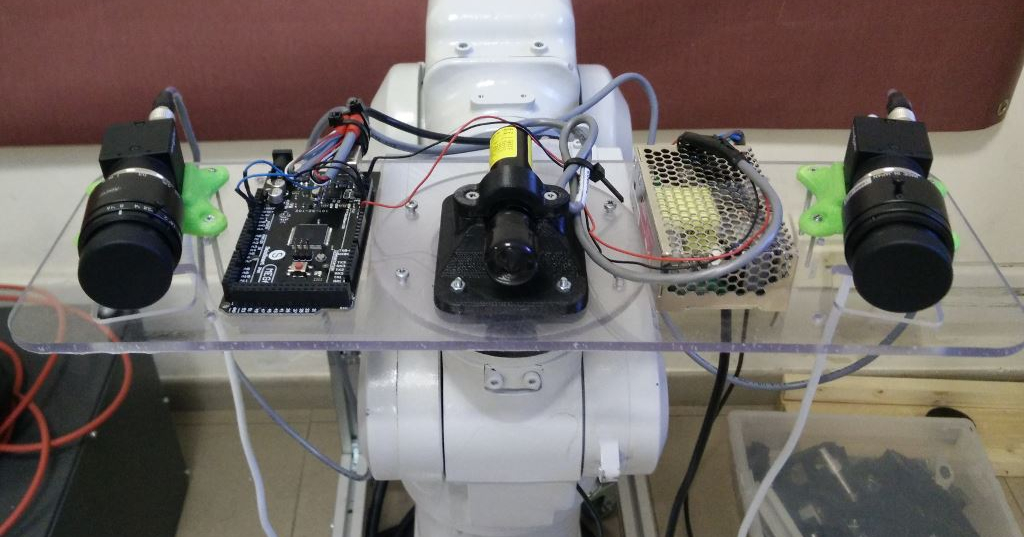
\includegraphics[width=0.8\textwidth]{figures/3_raw_dataset/fs_sensor_0}
    \caption{\textbf{FlexSight Sensor Detail}. From left to right: right high-resolution pointgray camera, arduino controller, pseudo-random laser projector, AC adapter, left high-resolution pointgray camera.}
    \label{fig:fs_sensor_0}
\end{figure}

\subsection{Microsoft Kinect 2 and Intel Realsense SR300}\label{subsec:raw_setup_kin&realsense}
On top of the FlexSight sensor, two commercially available 3D sensors have been mounted, namely a Microsoft Kinect 2 RGB-D sensor and a Intel Realsense SR300. Both the commercial sensors provided already registered depth and rgb images at low and high resolution respectively.

\begin{itemize}
	\item \textbf{RGB images}: \emph{1920x1080 px} for both the sensors.
	\item \textbf{Depth images}: \emph{512x424 px} for Microsoft Kinect 2 and \emph{640x480} for the Intel Realsense SR300.
\end{itemize}

Moreover, the two sensors have been chosen because they provide different features and can be of major interests for other commercial and common usages. In particular, the Intel Realsense SR300 is a so called \emph{short range} sensor, in the sense that its depth estimation is accurately working in short range, namely $0.2m$ to $1.5m$. While the Microsoft Kinect 2 provides wider range, namely $0.8m$ to $4.5m$.

\section{Acquisition Procedure}\label{sec:raw_acquisition_procedure}
All the scenes of the RAW Dataset have been acquired following a rigid and specific protocol. In particular, we have defined a set of camera poses by sampling a set of different semi-sphere in the range of $(85cm, 95cm)$ from the surface where the objects are placed. From the set of all the extrapolated poses we then developed a automatic collision-check procedure that eliminated all the poses where the robot body and the experimental FlexSight Sensor collide with the any of the elements of the cell.

At the end of the first automatic pose check procedure, more than 500 poses have been selected, then we manually tested all those poses and manually double checked all obtaining at the end 465 different camera poses.

With the list of all the poses and the robot and sensor setup safely working we started the acquisition of the 15 scenes of the dataset. The acquisition of each single scene was divided in two separated steps:

\begin{itemize}
	\item \textbf{FlexSight + Realsense Acquisition}: in this phase we only acquired images and depth images from the FlexSight sensor and the Intel Realsense SR300.
	\item \textbf{Kinect 2 Acquisition}: in this phase we only acquired images and depth images from Microsoft Kinect 2.
\end{itemize}

This separated sequence was decided in order to solve the laser interference among the two commercial sensor, the Microsoft Kinect 2 and the Intel Realsense SR300. Since those sensors are basically structured light based sensors, they work with internal laser patterns projectors, and they basically work in the same frequency ranges, that is why we experienced some interference in the depth images of both and decided to completely turn off the other sensor while the first was performing the acquisition.

For the FlexSight sensor we also split the acquisition in two different phases, namely with and without the projected laser pattern. Moreover, for each frame acquisition we took 4 different images that differs only for exposure time of the two cameras, namely $800{\mu}s, 2400{\mu}s, 10000{\mu}s$ and $52000{\mu}s$. In this way we can provide to all the future users of the RAW dataset the possibility to work both with the individual acquisitions or performing some HDR image manipulation using all the 4 acquisitions. An example of acquisition sequence from the FlexSight sensor is given in Figure \ref{fig:fs_sensor_sequence}.

\begin{figure}
    \centering
    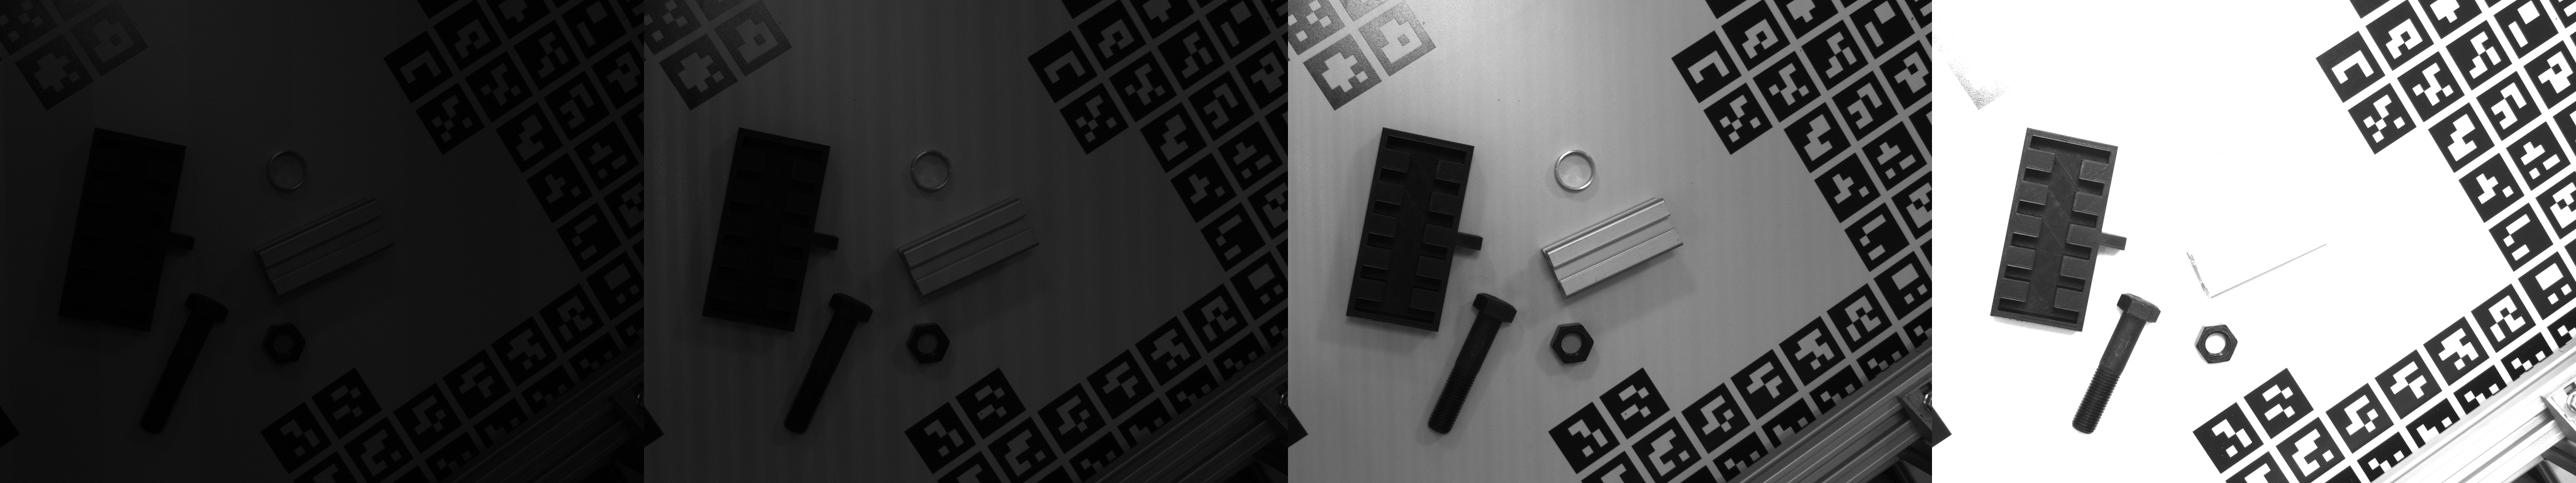
\includegraphics[width=\textwidth]{figures/3_raw_dataset/fs_sensor_sequence}
    \caption{\textbf{FlexSight Sensor Acquisition Sequence}. From left to right: the acquisitions with $800{\mu}s, 2400{\mu}s, 10000{\mu}s$ and $52000{\mu}s$ respectively.}
    \label{fig:fs_sensor_sequence}
\end{figure}

\section{Ground Truth Estimation Protocol}\label{sec:ground_truth_estim}
To do ...

\subsection{Labelling tool}\label{subsec:raw_labeltool}
To do ...

\subsection{Pose Propagation Pipeline}\label{subsec:pose_propagation}
To do ...